
%%%%%%%%%%%%%%%%%%%%%%%%%%%%%%%%%%
% Document class
%%%%%%%%%%%%%%%%%%%%%%%%%%%%%%%%%%
\documentclass[letterpaper,twocolumn,fleqn]{article} 

%%%%%%%%%%%%%%%%%%%%%%%%%%%%%%%%%%
% Packages
%%%%%%%%%%%%%%%%%%%%%%%%%%%%%%%%%%
\usepackage{ist,amsfonts, amsmath, color, amsthm, array}
\newtheorem{theorem}{Theorem}
\newtheorem{corollary}{Corollary}
\newtheorem{lemma}{Lemma}
\newtheorem*{remark}{Remark}

% add other packages here

\pagestyle{empty}                % no page numbers is default


%%%%%%%%%%%%%%%%%%%%%%%%%%%%%%%%%%
% Title and Authors
%%%%%%%%%%%%%%%%%%%%%%%%%%%%%%%%%%

\title{End-to-End Learning of Hierarchical Watersheds}
\author{
 Beate G. Zimmer, Dept. of Mathematics and Statistics, Texas A\&M University-Corpus Christi, Corpus Christi, TX 78412\texttt{ beate.zimmer@tamucc.edu} \\
 Venkatesh Jatla, Department of Computer Engineering, University of New Mexico, Albuquerque, NM 875XX \texttt{ venkatesh.jatla@gmail.com} \\
 Quan Nguyen, Department of Computer Science, University of Texas at Arlington, Arlington, TX 76019 \\\texttt{ remrace@gmail.com} \\
 Reid B. Porter, Computational and Computer Science Division, Los Alamos National Laboratory, Los Alamos, NM 87545 \texttt{ rporter@lanl.gov}
  }

\date{} % date has an empty field.

% correct for bad hyphenation here
\hyphenation{}

%%%%%%%%%%%%%%%%%%%%%%%%%%%%%%%%%%
% Begin document
%%%%%%%%%%%%%%%%%%%%%%%%%%%%%%%%%%
\begin{document} 

\maketitle 

\thispagestyle{empty} % prevents the first page to be numbered

%%%%%%%%%%%%%%%%%%%%%%%%%%%%%%%%%%
% Abstract
%%%%%%%%%%%%%%%%%%%%%%%%%%%%%%%%%%

\begin{abstract}

Over the last decade there has been much progress and success in end-to-end learning, where application level performance metrics, in combination with large training sets, are used to optimize deep neural network pipelines for the task at hand. This success has been most significant in solving image and pixel classification problems where inference (test-time prediction) has been fairly simple e.g. a forward pass function evaluation. There is now much interest  in extending this success to a wide variety of problems where inference is more complex, such as supervised segmentation (and clustering). This interest is partly fueled by the training sets that have been made available, and partly because the learning problem has become better defined in terms of deep structured output prediction. 

In this paper we present an end-to-end training method for Hierarchical Watershed segmentations and the Rand Error. Our approach combines deep neural networks for modeling dependencies between pixels and deep multi-layered graphical models for modeling dependencies in predicted segmentations. The combined model is computationally efficient and can be efficiently trained to minimize a convex surrogate of the Rand Error. We believe our approach extends end-to-end learning of the Rand Error to structured outputs that are deeper than previous efforts. This means our approach benefits from fewer parameters and fewer application specific design choices.
\end{abstract}


% keywords can be removed
%\keywords{Watershed cuts \and Connected Components \and Hierarchical segmentation}


\section{Introduction}

Image segmentation is a fundamental task in image and video processing that has wide ranging applications. Segmentation has traditionally been an unsupervised problem, that is similar to, and shares many solution methods with, clustering and graph partitioning. However, with the improvements in performance that have been achieved on image classification benchmarks with supervised deep neural networks, there has been increasing interest in developing supervised methods that can provide similar improvements in segmentation. 

A related supervised problem that has received extensive attention is semantic segmentation. In this problem the training data is in the form of pixel labels and the labels often define object types or categories within the image. These labels are very similar to the labels used in image classification and so one solution is to simply use image classification solutions to solve the pixel classification problem \cite{Long2015}. In recent years, semantic segmentation benchmarks have started to include additional pixel level labels that identify instances, and this has led to a variety of methods that build on semantic segmentation solutions to differentiate the multiple instances of a particular object category. Solution methods to this problem begin to overlap with the methods developed here. 

In this paper we focus on segmentation problems that are closer to clustering than to classification. The pixel labels used in training are identifiers for a segment, partition, or cluster, and do not correspond to any particular object category. This type of training data appears most often in analysis of imagery collected in biomedical, material science and other scientific disciplines. In these images the pixel or object category, can be the same across the entire image and is therefore left unspecified, and segmenting the image to differentiate instances is the primary objective. In material science these instances might correspond to different crystals, or grains, of a material. In biomedical applications these instances might correspond to different cells. We note that in most applications there exists a combination of object category and instance information that is of interest and that eventually most applications would benefit from solution methods that can predict both. However, focusing on the instance problem leads to different methods and different prior work compared to the methods that have been extended from the classification problem. In this paper we focus purely on the instance problem and we discuss how the methods developed could be extended to predict categories in future work.

The general framework in which we develop solutions to segmentation, and relate it to other work, is deep structured output prediction. We associate a set of random variables $X=(x_1,x_2,...,x_N), x_i \in \mathbb{R}^D$ with an input image of $N$ pixels. We associate another set of discrete random variables $Y=(y_1,y_2,...,y_N),y_i \in \{1,2,\ldots,N\}$ with the output segmentation. Solution methods will define various energy functions that have parameters $w$ (that we learn in training), and produce segmentations by solving the inference problem: $\widehat{Y} =\hbox{argmin}_{Y}E_{w}(X,Y)$. 

The pixel and image classification problems mentioned earlier typically use deep multi-layered networks to incrementally model the dependencies between input variables $X$ and predict output variables independently $\widehat{y_i} = E_{w}(X)$. More recent work in semantic segmentation couples deep networks with conditional random fields (CRF) \cite{Sutton2011} to incorporate output dependencies \cite{Chen2014}. A common theme is to map approximate inference methods into feed forward layers in the final stages of the network \cite{Zheng2015}. Semantic segmentation methods often model dependencies between output variables, but the loss function used in training is typically the same convex surrogate for classification error that is used in pixel classification. 

Methods for supervised segmentation have traditionally treated learning and segmentation as independent steps where classifiers can be trained to minimize classification error \cite{Arbelaez2011}. We note a more recent approach to training edge classifiers includes modeling dependencies between output variables \cite{Dollar2013}. Turaga et al.\cite{turaga} was perhaps the first to train a network with output dependencies to minimize a segmentation loss function. Their approach is analogous to semantic segmentation methods that feed deep networks into CRF type output layers, and train the end-to-end system. In terms of deep structured output prediction, these methods can be described as deep in the input space, but shallow (single layer) in the output space. 

\begin{figure}[h!]
    \centering
    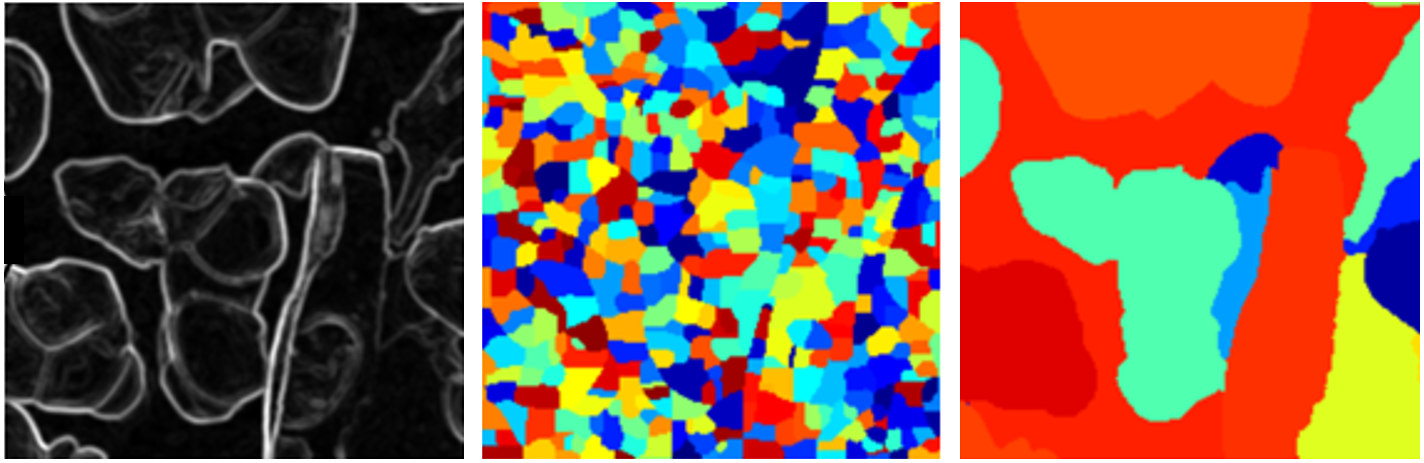
\includegraphics[height = 0.117\textheight]{Image_Hierarchy.png}
    \caption{The traditional hierarchical watershed is typically applied to an image gradient (left) and predicts segments (labels) in a two stage process that first oversegments (middle) and then merges into final segments (right).}
    \label{fig:image_example}
\end{figure}

In this paper we consider a number of traditional hierarchical watershed segmentation methods that are deep in the output space. As shown in Fig. 1 these methods produce segmentations in two steps. The first step partitions the regular grid of pixels into super-pixels. The second step partitions an irregular and data dependent set of super-pixels into the final segments. These traditional methods incrementally model output dependencies with multiple layers and can potentially capture long range, and multi-scale dependencies, that a single layer cannot. 

In the next Section we will reintroduce a number of hierarchical watershed segmentations in terms of multi-layered energy functions. We then describe this paper's main contribution, which is a computationally efficient, end-to-end learning method that directly minimizes a segmentation loss function. In our experiments we investigate some of the tradeoffs in the approach as well as its performance using a biomedical benchmark dataset.

\section{Single Layer Segmentation}

A large number of segmentation methods can be described in terms of a single layer graph $G = (V, E)$. The vertices ($V$) are associated with a set of $N$ image pixels $X=(x_1,x_2,...,x_N), x_i \in \mathbb{R}^D$ and a set of discrete labels $Y=(y_1,y_2,...,y_N),y_i \in \{1,2,\ldots,N\}$. The edges $(E)$ associate unordered pairs of vertices (typically the 4, or 8, closest neighbors in the image grid) and a set of real valued edge affinities $A=(a_{1,2},a_{2,3},...,a_{N-1,N}), a_{ij} \in \mathbb{R}$. Throughout this paper we will assume that these affinities are unique, since for some methods, this will guarantee that the segmentation is unique. In this section we will assume that these affinities are provided and will describe fixed scalars real valued Since we will eventually learn the edge affinities this assumption is typically not a serious restriction. Segmentation is defined as finding a labeling of the graph that minimize an energy function, which is typically a sum of terms associated with each edge:
\begin{equation}
    \widehat{Y} =\hbox{argmin}_Y\sum_{e_{ij}\in E} g(y_i, y_j, a_{ij})
    \label{Eq:1}
\end{equation}
A large number of segmentation and clustering algorithms can be defined through the appropriate choice of $g$ and $A$. The best $g$ depends on the application, and finding the $g$ that works best in a specific application is often challenging. In many cases a practitioner will try  several different choices (different algorithms) and pick the method with results that best serves their purpose. 

One of the most general energy functions that has been investigated for segmentation and clustering is known as Correlation Clustering \cite{Bansal2004} and it uses the edge function in Eq.~\ref{Eq:3}: 
\begin{equation}
    g(y_i, y_j, a_{ij}) = I(y_i \neq y_j)\cdot a_{ij}
    \label{Eq:3}
\end{equation}

In this setting  the edge weights denote correlations and Correlation clustering tries to maximize agreements by joining positive edges and minimize disagreements by cutting negative edges. Correlation clustering is NP complete (i.e. there is no fast way to solve Eq. \ref{Eq:1} with Eq. \ref{Eq:3}) and so researchers have investigated more restrictive edge functions where solutions can be found efficiently. 

Perhaps the most widely used example of this is known as graph-cuts, and it restricts the function by only considering binary labels $y_i \in \{0,1\}$ and requiring affinities to satisfy a sub-modularity constraint. Note, the term graph-cuts is also sometimes used to describe an approximate inference method that solves the multi-label problem by solving a sequence of (tractable) binary problems.In the next section we introduce other examples of tractable edge functions that solve the multi-label problem $y_i \in \{1,2,...,N\}$ directly, but restrict the affinity function in other ways. 

\subsection{Connected Components}
\label{subsec:cc}

We define Connected Component (CC) segmentation as finding the labeling that minimizes Eq.~\ref{Eq:1} with the edge function in Eq.~\ref{Eq:4}: 
\begin{equation}
    g(y_i, y_j, a_{ij}^*) = I(y_i \neq y_j)\cdot\max_{P\in\mathcal{P}_{ij}}\left( \min_{e_{rs} \in P} ( a_{rs} ) \right) 
    \label{Eq:4}
\end{equation}
where $\mathcal{P}_{ij}$ denotes the set of all paths from vertex $i$ to vertex $j$. In Eq.~\ref{Eq:4} each affinity is potentially replaced by the affinity associated with a different edge in the graph ($a_{ij}^*$). The \emph{maximin} procedure first selects a minimum affinity along each path between between vertices $i$ and $j$ and then chooses the (minimum) affinity that is a maximum in the set of all paths. A labeling that minimizes Eq.~\ref{Eq:1} for the edge terms in Eq.~\ref{Eq:4} can be found efficiently since the potential for disagreements, with respect to transitivity, has been removed. In correlation clustering  this labeling is called a perfect clustering and can be found with a simple two-step procedure:
\begin{enumerate}
\item Cut  edges that have maximin affinities below zero.
\item Run a connected component procedure on the remaining sub-graphs to obtain vertex labels.
\end{enumerate}

The two-step CC procedure highlights the fact that labels that minimize Eq.~\ref{Eq:4} depend on the sign of the edge affinities, but not on their magnitudes. Although the labels are not constrained in any way, the MaxiMin procedure appears to be a more restrictive constraint than sub-modularity, and this also manifests in $O(N)$ run-time for connected component segmentation  compared to $O(N\log N)$ for graph-cuts\cite{Schmidt2009}. 

Connected Component segmentation is closely related to single linkage clustering and the minimum spanning tree (MST) of the affinity graph. On the left in Figure 2 we illustrate CC segmentation for a hypothetical 1-Dimensional, 10 pixel image. The MST edges of the affinity graph are illustrated as squares, and CC segmentation corresponds to a horizontal cut of the MST at some threshold. Note, that in Eq.\ref{Eq:4} the threshold was assumed zero. 

\begin{figure}[h]
    \centering
    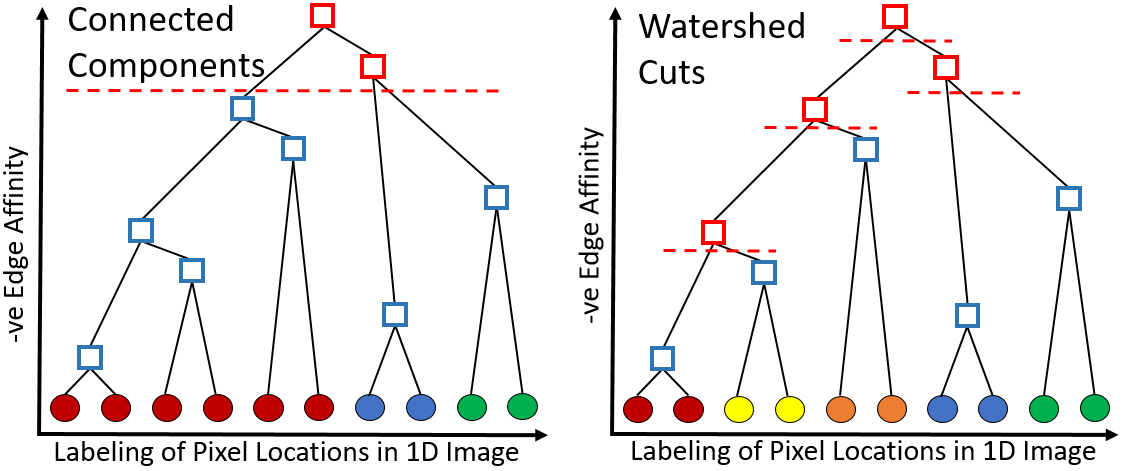
\includegraphics[height = 0.15\textheight]{cc_ws_tree.png}
    \caption{Segmentation as cuts of the MST Left) Connected Components and Right) Watershed Cuts.}
    \label{fig:inferning_threshold}
\end{figure}

\subsection{Watershed Cuts}
\label{subsec:ws}
The Watershed-Cut (WS) segmentation can also be defined in terms of an edge function, but in this case it involves raising affinities to an infinite power Couprie \cite{Couprie2011}. In \cite{Cousty2009} the relationship between watershed cuts and the Minimum Spanning Forrest (MSF) is described. Local minima of the affinity graph induce separate sub-trees corresponding to watershed basins. As shown on the right in Figure 2, these sub-trees can also be identified in the MST. Unlike the horizontal cut used in CC segmentation, Watershed Cuts segmentation is a multi-level cut that is defined by local properties of the affinity graph. Specifically, to determine the Watershed Cuts we calculate auxiliary weight for each (MST) edge that is computed only over the adjoining edges. If $i$ is a vertex, let $N_i$ denote the set of all neighboring vertices and let $a_{ij}$ denote the affinity of edge $e_{ij}$ between vertices $i$ and $j$. We define an  auxiliary affinity:
\begin{equation}\label{eq:LocalMinMax}
a_{ij}^*=\min\left( \max_{k\in N_i\setminus\{j\}}a_{ik},\max_{k\in N_j\setminus\{i\}}a_{kj}\right).
\end{equation}
If $a_{ij}^*<a_{ij}$ then on at least one side of the edge $e_{ij}$, all adjoining edges have lower weights and in that direction no all-uphill path to a local maximum exists. This puts the edge $e_{ij}$ in a watershed basin in the original notation of watershed cuts. In our case high affinities denote similarity and we do a watershed cut on the negatives of the affinities or we could say we consider hills and put the cuts at the bottom of the valleys between adjoining hills.
If $a_{ij}^*> a_{ij}$, then on both sides of edge $e_{ij}$ an uphill edge exists and we have a watershed edge (or identified a valley bottom). The watershed cut can be calculated by removing all such edges and then finding the connected components of the remaining sub-graphs. 

CC segmentation tests if an edge is part of the cut by comparing each edge affinity to a threshold which we have so far assumed to be set at 0. Note that the WS segmentation also tests each edge, and could also have a threshold introduced as: $a_{ij}^* - a_{ij} > \theta$.  

\subsection{Constrained Correlation Clustering}
\label{subsec:ccc}

The CC and WS segmentation methods have efficient algorithms for minimizing restricted multi-label energy functions but, they are potentially too restrictive. One way to make the methods more flexible, and more useful in a wider range of applications, is to use learning to optimize affinities. This will be  described in detail with respect to Supervised Segmentation. The alternative is to find ways to improve the segmentation while maintaining the computational efficiency. Traditional hierarchical segmentation methods are perhaps the best example of this and they produce better segmentations by using multiple single layer segmentations in combination. However, before moving to multi-layer solutions, we note that it is also possible to increase the flexibility of single layer methods while maintaining computational efficiency.

In prior work we observed that the threshold parameter in CC and WS segmentation is often a critical parameter that can have a significant impact on generalization \cite{Nguyen2019}. Our solution was to move threshold selection into the segmentation method itself so that it could be adapted during inference to the image at hand. Specifically, we define a set of partitions $\Omega = \left(\widehat{Y}^1, \widehat{Y}^2, ..., \widehat{Y}^N\right)$ that minimize connected component segmentation after a predefined set of offsets $\left(\theta^1, \theta^2, ..., \theta^N\right)$ have been applied:
%\begin{equation}
%    \widehat{Y^n} =\hbox{argmin}_Y\sum_{e_{ij}\in E} I(y_i \neq y_j)\cdot \max_{P \in\mathcal{P}_{ij}}\left( \min_{e_{rs} \in P} %\left( a_{rs} - \theta^n \right) \right)
%    \label{Eq:5}
%\end{equation}
\begin{equation}
    \widehat{Y}^n =\hbox{argmin}_Y\sum_{e_{ij}\in E} I(y_i \neq y_j)\cdot (a_{ij}^*-\theta^n)
   \label{Eq:5}
\end{equation}

This is equivalent to thresholding the maximin affinities at values other than $0$ in the two-step procedure. To obtain the final labeling, we pick the partition from the set that minimizes the correlation clustering energy function:  
\begin{equation}
    \widehat{Y} =\hbox{argmin}_{\widehat{Y}^n \in \Omega} \sum_{e_{ij}\in E} I(\widehat{y_i}^n \neq \widehat{y_j}^n)\cdot a_{ij}
    \label{Eq:6}
\end{equation}

Equation~\ref{Eq:6} solves correlation clustering efficiently by only considering $N$ partitions defined by connected components at predefined thresholds. In the upcoming section on supervised segmentation we describe how a modification of Kruskal's MST algorithm can be used to evaluate Eq~\ref{Eq:6} in $O(N\log N)$ time in most cases. In related work, a segmentation method called the Mutex watershed was recently introduced and has several similarities to the approach we have described. Their approach also adapts Kruskals algorithm for watershed segmentation so that it includes negative affinities and also maintains the $O(NlogN)$ efficiency in most cases \cite{Wolf2019}. 

\section{Hierarchical Segmentation}

A large number of hierarchical segmentation methods can be defined in terms of two layer graphs involving Connected Component (CC) and Watershed Cuts (WS) energy functions in different ways. A conceptual view of how these methods work is shown in Fig. 3. The segmentation labels define super-pixels, which are then associated with vertices in a second layer graph. Connectivity of super-pixels define edges in the second layer graph and a second energy associated with the graph is minimized to find the final labeling. Multi-layer  segmentation methods can be formulated as a single graphical model with a recursive energy function. For example, we define a two-layer model as: 
\begin{equation}
    E(Z,Y,X)=\sum_{e_{ij}\in E_Y}▒〖g_2 (z_i,z_j,X,Y) 〗+\sum_{v_i\in V_Y}▒\sum_{e_{mn}\in v_i}▒〖g_1 (y_m,y_n,X) 〗
    \label{Eq:recurse}
\end{equation}

However, this formulation has not been explicit in the segmentation literature and perhaps because of this, minimizing the function is almost always one layer at a time, in a greedy feed forward fashion. In this paper, we also focus on the greedy minimization approach. However, knowing when this is exact, and when it is not, and comparing to other minimization strategies \cite{corso} would be an interesting direction for future work. 

\begin{figure}[h]
    \centering
    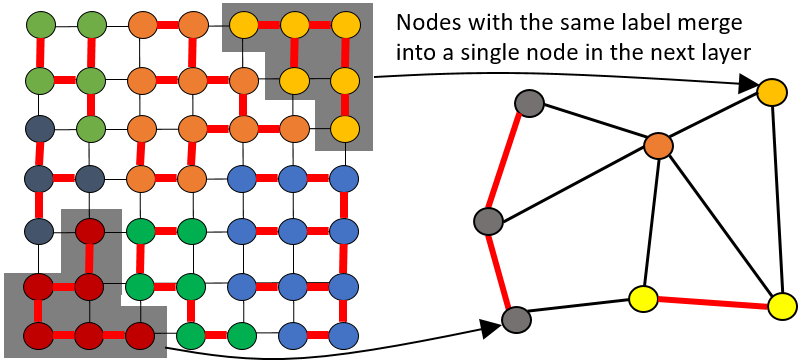
\includegraphics[height = 0.163\textheight]{Two_Hierarchy.png}
    \caption{Hierarchical watershed segmentation can be visualized as a two layer graph.}
    \label{fig:inferning_threshold}
\end{figure}

In the next few sections we describe a number of two layer segmentation methods that have appeared in the traditional hierarchical watershed segmentation literature. The structure of these multi-layered graphs is data adaptive and is able to capture longer range dependencies between label variables than single layer graphs based on the regular pixel grid. 

\subsection{WS-CC Hierarchies}
\label{sec::WScc}

One of the most widely used hierarchical watersheds first segments the pixel graph by minimizing the WS energy. In traditional implementations, affinities are gradient estimates and the labeling identifies edge respecting local minima which is typically very over-segmented. The labeling defines the second layer graph (super-pixel graph) and the final labeling is obtained by minimizing the CC energy \cite{mangan}. A key design choice in the traditional implementation is the affinity used in the second layer graph. Many different \emph{features} have been suggested including affinities from the first layer, the depth, the area, and the volume. In this paper we use a fixed second layer affinity function as well (the depth) but this is a choice that could potentially be left to learning. 

The depth (or height) is defined as the difference between.... For each original edge $e_{ij}$ between two super-pixels, let $a_i$ denote the lowest (or highest) affinity in the segment that contains vertex $i$.  We define the depth as: 
\begin{equation} 
 d_{ij}=\min \left( a_i, a_j\right)-a_{ij}
\end{equation}
which is the minimum hill height on either side. All of the depths are positive and the goal is to merge the lowest hills with their neighbors, whereas connected components merges the highest affinities. In traditional implementations, a variety of heuristics have been proposed to select the depth threshold for merging. It is also very common to make this threshold a user controlled parameter and because the connected component segmentation is computationally efficient, and operating on a small number of nodes in the super-graph, this control can be interactive and set by user's visually. 

In this paper, we set the threshold automatically by using the Constrained Correlation Clustering method. However, before we can apply this method we require affinities that are both positive and negative. Our solution is to shift the depth values by an offset defined by a simple order statistic of the super-graph's edge depths. In  experiments we  found using the $75^{th}$ value worked well over a large number of applications. However, Figure~?? in our experiments illustrates that the method is fairly robust and provides similar performance over a wide range from the $50^{th}$ to the $80^{th}$ sample. Note, since we would like to merge small depth values first we must flip the sign of the affinity and choose the $25^{th}$ sample to be consistent with our previous definition of Connected Components which we denote as $d_{(25)}$. With this offset we define new affinities for the CC segmentation as $d^{*}_{ij}=d_{(25)}-d_{ij}$.

With the super-graph affinities now defined, and shifted, we find the connected component threshold that minimizes the Correlation Clustering objective. The thresholds that define the set of partitions we consider are defined by the adjusted MST depth values. That is, we consider thresholds that lie half way between consecutive $d^{*}_{ij}$ values that have been sorted (and assumed to be unique). 

\subsection{Waterfall Hierarchies}
 Meyer in \cite{Meyer2015} described a waterfall hierarchy consisting of a sequence of watershed cuts (WS-WS).  Generally  a watershed cut oversegments an image. Instead of using CC segmentation in the second step, we simply repeat WS segmentation on the super-graph. In this case the affinity associated with each super-graph edge is the original affinity of the edge that first connects the two basins. The modular nature of the Waterfall segmentation suggests we can continue this process and the total number of WS segmentations (the number of layers in the graph) required to arrive at one segment is image dependent. In addition, because affinities do not have to be recalculated, the full Waterfall can be calculated in a single pass of the MST. In future work we plan to compare learning WS-WC hierarchies with learning Waterfall hierarchies. Assuming we use a threshold of $0$ in WS segmentation, the Waterfall introduces a new threshold which corresponds to the number of WS segmentations that we use. In comparison to CC segmentation, we expect the number of potential thresholds to be much smaller, which means the Waterfall is probably a more constrained (but potentially more robust) hierarchy compared to WS-CC. 
 
\subsection{CC-WS Hierarchies}

In previous work we investigated a family of multi-layered hierarchies, that we called Deep Segmentation Networks, that include Waterfall and WS-CC hierarchies as special cases as well as other combinations that include CC segmentation on the pixel graph, followed by WS segmentation on the super-pixel graph. By the following argument we can guarantee that the CC-WS hierarchy generates a different set of segmentations than the CC-CC segmentation. All neighboring edges of the super-graph edge with the highest affinity must be smaller guaranteeing that $a_{ij}^*< a_{ij}$ and the edge will not be cut. For the second highest super-graph edge, at least one side has neighbors that are all lower, guaranteeing that it cannot be cut as well. Since all MST edges are potential cuts in CC segmentation, the potential segmentations will be different. 

\section{Supervised Segmentation}

Supervised segmentation starts with a training set of $M$ (image, label-image) pairs $S={(X(1),Y(1)), (X(2), Y(2),...,(X(M),Y(M))}$. Each label-image $Y(m) = (y_1, y_2, ..., y_N)$ has a label associated with each pixel and represents the target segmentation for the image $X(m)$. In supervised classification labels correspond to classes, or categories, and the misclassification error is the typical performance measure. When their is a label for each pixel, the problem is often called semantic segmentation. However, we prefer the name pixel classification, since the problem is closer to classification than segmentation. 

We use the term segmentation for the case when labels are unique identifiers for the segment, partition, or cluster, and the actual value of the identifier is arbitrary. Note, that unlike classification, the number of distinct labels $y_n\in{1, 2, 3, ...}$ can vary from one image to the next. Although, the maximum number of potential labels is the same for all images and equal to the number of pixels $N$. 

To estimate the performance of a predicted segmentation ($\widehat{Y}$) with respect to a ground truth segmentation ($Y$) requires a quantity that is independent of the identifiers used. One of the first quantities proposed to evaluate labels of this form is the Rand Index \cite{Rand}. Instead of counting the number of pixels labels that are mistakes, it counts the number of pixel pairs that are mistakes. To determine if a pixel pair is a mistake we define two new variables. We assign $y_{i,j}=1$ when $y_i = y_j$ and zero otherwise. We assign $\widehat{y}_{i,j}=1$ if $\widehat{y}_i = \widehat{y}_j$ and zero otherwise. The Rand Error (RE) is a minor modification of the Rand Index that counts the number of pixel-pair mistakes over all pairs: 

$$RE(Y,\widehat{Y})=\binom{N}{2}^{-1} \sum_{V\times V } \left(y_{ij}\neq\widehat{y}_{ij}\right)$$

Note, that counting the pixel pair mistakes over all pixel pairs in the graph is different to counting the pixel pairs over all edges in the pixel graph. In 2D and 3D image segmentation, the graph based Edge Error (EE) typically involves a much smaller number of terms:

$$EE(Y,\widehat{Y})=\frac{1}{\vert \cal{E}\vert} \sum_{e_{ij}\in\cal{E} } \left(y_{ij}\neq\widehat{y}_{ij}\right)$$

Unless the graph is fully connected this error cannot capture the long range dependencies that the Rand Error can.

\subsection{Learning Connected Components}

Turaga \cite{Turaga09} \cite{Turaga10} observed that the gradient of the CC segmentation can be estimated through the maximin edges that we introduced in Eq.~\ref{Eq:4}. In our prior work we suggested a modification of Kruskal's algorithm \cite{Kruskal} to construct a maximum spanning tree and keep track of how many new correct (positive) pixel-pair labels, $\#\hbox{same}$, and how many new false positive (negative) pixel-pair labels, $\#\hbox{diff}$, are introduced with each new MST edge. Initially each vertex is considered a segment with a membership array of all zeros, except for a one in the ground-truth label associated with that vertex. Greedily adding an MST edge to the tree merges segments and their membership arrays are added to produce a membership array for the new segment created. For the $n$-th edge added to the MST, $\#\hbox{same(n)}$ is calculated by the dot product of the the membership vectors associated with the segments it connects:
\begin{equation}
\#\hbox{same}(n)=m_1\bullet m_2    
\end{equation}
The corresponding $\#\hbox{diff}(n)$ for the edge is: 
\begin{equation}
\#\hbox{diff}(n)=\Vert m_1\Vert_1 \Vert m_2\Vert_1-m_1\bullet m_2.
\end{equation}

The segments in the CC segmentation are formed by a spanning forest consisting of the MST edges of positive affinity (or affinities above a chosen threshold). If we assume we have $T$ MST edges above threshold, then the Rand error of the resulting segmentation is the number of missing correct connections between pairs of vertices, plus the number of false connections already made, divided by the total number of vertex pairs:
\begin{equation}
\label{eq::rand}
\begin{split}
RE(Y,\widehat{Y}, T)&=\binom{N}{2}^{-1}\left(\sum_{n=1}^T \#\hbox{diff}(n)+\sum_{n=T+1}^{N-1} \#\hbox{same}(n)\right)\\
&= C + \binom{N}{2}^{-1}\left(\sum_{n=1}^T \#\hbox{diff}(n)- \#\hbox{same}(n)\right)\\
\end{split}
\end{equation}
where the constant $C$ is independent of $T$. 
Working with just the MST edges instead of all possible pairs reduces the complexity of calculating the Rand Error from $O(N^2)$ to $O(N-1)$. 

\subsubsection{Surrogate Loss Functions}
In the last section we showed how the Rand Error for CC segmentation can be expressed in terms of a new training set for a binary classification problem on MST edges. Specifically, each example $(X(m),Y(m))$ produces a training set with multiple copies of each MST edge. The number of times a particular MST edge appears in the training set with a label of $+1$ is $\#\hbox{same(n)}$. The number of times it appears with a label of $-1$ is $\#\hbox{diff(n)}$. This new problem is better computationally than the original problem because there are only $N-1$ unique examples. However, the training set is conflicted and this introduces some new challenges depending on the learning method used.

We consider the new problem as a weighted classification problem. We assign the MST edge a label of $+1$ whenever $\#\hbox{same(n)} >\#\hbox{diff(n)}$ and a label of $-1$ otherwise. Ideally, each weight would represent how much the edge contributes to the overall Rand Error. However, because of the conflicts in the training set, this is difficult to estimate and we must balance two terms: 1) the fraction of the Rand Error that the edge is responsible for, with 2) how much each edge is conflicted. We estimate the second term in terms of purity:
\begin{equation}\label{eq:purity}
P(n) = \left\vert \frac{\#\hbox{same(n)}-\#\hbox{diff(n)}}{\#\hbox{same(n)}+\#\hbox{diff(n)}}\right\vert
\end{equation}
Purity takes the value 1 for perfect edges that have Rand Error contributions that are all the same, or all different. An edge that has an equal number of $\#\hbox{same}$ and $\#\hbox{diff}$ counts has a weight of $0$. Purity gives greater weight to edges that are less conflicted, but does not capture the total number of terms that the edge will contribute to in the Rand Error. Said another way, purity does not penalize the false negatives, which means the segmentations produced will tend to be over-segmented. Our solution is to simply multiply the purity of each edge by the total Rand Error which does include the false negatives. 

The final component required for the Rand Loss function is to choose the convex surrogate for the weighted binary classification problem. It could be any of the standard choices e.g. squared error, logistic loss, or hinge loss. Here, we describe the surrogate problem in terms of the squared error, which is what we use in our experiments. 
\begin{equation}
    \label{eq:weighted_classification}
    RL(Y, A) = \sum_{n\in MST}{W(n) \cdot \left(a_n-\ell(n)\right)^2},
\end{equation}
where
\begin{equation}\label{eq:label}
\ell(n) = sign(\#\hbox{same(n)} -\#\hbox{diff(n)})
\end{equation}\\
and
\begin{equation}\label{eq:weight}
W(n) = P(n)*RE(Y,\widehat{Y},T)
\end{equation}\\
Note, we know $T$ after applying a real valued threshold that lies between the $T^{th}$ and $(T+1)^{th}$ MST edge. 

\subsubsection{Learning Watershed Cuts}
In prior work showed how the approach described above can be easily extended to learning watershed-cuts \cite{PorterOyenZimmer15}. It is based on the observation that a WS segmentation can be calculated locally through the use of minimax weights $A_{ij}^*$ defined in equation  \ref{eq:LocalMinMax} in addition to the original weights $A_{ij}$. The $A_{ij}^*$ calculation is only based on the immediate neighboring edges and an edge is a watershed edge if $A_{ij}^*>A_{ij}$. By modifying the affinity graph edge weights $A_{ij}'=A_{ij}-A_{ij}^*$ the algorithm of the previous section will give counts for how many correct an how many incorrect connections an edge makes as it is added to the spanning forest for the watershed cut.

\subsubsection{Learning Constrained Correlation Clustering}

The correlation clustering energy of CC or WS segmentations can also be calculated efficiently with another minor extension to the Kruskal algorithm used to calculate the Rand Error. The initial correlation clustering energy for no edges is the sum of all affinities in the graph. Adding an edge to the MST joins two segments. When two segments are joined, we need to subtract the affinities of any edges between the two segments from the previous correlation clustering energy. To make this efficient we use pointer cycles to keep track of vertices within each segment as we build the MST. While this is $O(N^2)$ in the worst case, in practice we found that the lowest correlation clustering energy occurs well before the end of the MST where segments are typically the largest. By stopping early we were able to find minimum correlation clustering energies at small additional cost to the original $O(NlogN)$ algorithm. Note, the same algorithm is used at test time, but in that case there is no Rand Error calculation. 

\subsection{Learning Hierarchical Watersheds}
\label{subsec:RE Hierarchy}
The hierarchical segmentation described in Section~\ref{sec::WScc} uses two passes of the Kruskal algorithm to calculate the Rand Error. In the first pass we identify the watershed basins and accumulate the positive and negative counts associated with basin edges. Note that we don't consider the edges between watershed basins in this first pass which means we are ignoring the false negatives. The basin edges receive labels and weights as defined by Equation~\ref{eq:weighted_loss_meta}. We note that in the proposed weighting scheme the watershed basin edges do in fact include the cost of false negatives, since it is captured in the Rand Error of the final segmentation. 

In the second pass we continue to accumulate the positive and negative counts, but in the order defined by the depth in the super-pixel graph. Recall that the depth is a function of three edges: 1) the current super-pixel edge and 2\&3) the lowest (first) edges introduced in the watershed segmentation. This dependency suggests a possible reweighting of the basin edges, but we observed little improvement compared to simply ignoring the dependence (this is described more in Section ??). The super-pixel MST edges are assigned labels and weights according to Equation~\ref{eq:weighted_loss_meta} just like the pixel-graph MSF edges. During the second pass we also calculate the MST threshold that minimizes the correlation clustering energy. This threshold is then used to calculate final Rand Error of the super-pixel graph with Equation~\ref{eq::rand}. 

A recent work...  \cite{Turaga19} they claim to calculate a Rand error error based loss function through two passes through the affinity graph. In the positive pass all edges between segments are set to zero (or minus infinity if we have negative affinities?) and the errors of an MST of the new affinity graph are calculated. (This may calculate the false negatives?)  In a second pass all edges within segments are set to 1 (or plus infinity if affinities aren't normalized?) and the errors for an MST for this graph are computed. This may calculate the false positives? 


\subsection{Mapping Pixel Predictions to Edge Affinities}
\label{subsec:mapping}

We would like to use a deep neural network to produce the real valued affinities $a_{i,j}=f_w(X_{ij})$ in equation \ref{Eq:1}. Here, $X_{ij}$ is the subset of the image (could be the whole image) used by the neural network to determine if pixels $i$ and $j$ should be in the same segment, and $w$ are the parameters that are optimized to minimize the loss function during training. Currently, the most common approach is to use a traditional neural network where inputs and outputs are defined on the pixel grid. This means that the network output is more naturally interpreted as producing vertex affinities: $a_{i}=f_w(X_{i})$ which must be mapped somehow to edge affinities. 

Perhaps the most common mapping is to represent different sets of edges with specific network outputs. For example, for 2D, 4-neighbor graphs, the neural network is expected to produce two image-sized output channels. The first image is assigned to the horizontal edges and the second image is assigned to the vertical edges. Note, since there are only $(N-1)(N-1)$ edges of each type, the last row and column of each image is simply ignored. A third output channel is used for 3D voxel graphs. Additional output channels can also be associated with other sets of edges, such as longer range connections in different directions.

In our experiments we explored a simpler, more constrained mapping. We assume the network has one output and the edge affinity is the average of the vertex affinities associated with that edge. One advantage of this mapping is that the neural network architecture does not depend on the choice of graph structure. The mapping could also be generalized to map network outputs to irregular, data adaptive graphs, like the super-pixel graph. 

So far, we have described the mapping used in the forward pass. To train the network end-to-end we must also define the mapping for the backward pass. For the multi-channel mapping that we described first, we initialize zero valued label and weight arrays of the same size and number of channels as the network output. We then simply identify the channel and location in the array that is associated with each MST edge in Equation~\ref{eq:loss} and assign the label and weight calculated in Equations \ref{eq:label} and \ref{eq:weight}. The standard loss function in Equation \ref{eq:weighted_classification} can then be calculated and errors back-propagated with auto-differentiation or other mechanism. For the second mapping, the MST edges are easier to locate since there is only one network output but we must assign the associated label and weight to both of the edges vertices. 

\section{Experiments}
 
For experiments we use the training set for the ISBI 2013 challenge: 3D segmentation of neurons in electron microscopy images. Credit for generating these data goes to \cite{kasthuri2015}. The data set is a 8-bit grayscale, 1024x1024x100 pixels image cube of slices of an serial section scanning electron microspcopy 3D image of a of mouse cortex used for automatic segmentation of neurites in 3D.  The microcube measures 6 x 6 x 3 microns approximately, with a resolution of 6x6x30 nm/pixel. The image cube comes with a corresponding ground truth which has pixel level segment identifiers for all slices. We found that the "zero" label has special meaning in this dataset since there are multiple connected components with this value in the ground truth. To make it easier to apply our approach we gave each zero-valued connected component a unique label. We divide all images into non-overlapping sub images that are 128x128 pixels. This was purely to increase the number of experiments we could run with the resources we had and is not because of any fundamental size limit of our approach which is roughly $O(NlogN)$ in the number of pixels. 

Our first experiments investigate some of the design choices of our hierarchical watershed method. In these experiments, there is no learning, and we replace the raw image data with 2D probability maps of neuron membranes provided by \cite{ciresan2012deep}. These probability maps are produced by deep neural networks that won the ISBI 2012 challenge. They estimate a probability for each pixel as membrane or non-membrane and we treat this as if it were a traditional gradient estimate. We use the single channel mapping described in Section\ref{subsec:mapping} where the edge affinities of the pixel graph are simple averages of the associated pixels. In Figure~\ref{fig:offset_radius} we compare the average rand error of 25 images as we varied different meta parameters. Along the x-axis we varied the the correlation clustering offset which we typically leave at $0.75$. The different r-curves correspond to pixel graphs with different neighborhoods. For the $r=1$ curve each vertex has edges to its 9 closest neighbors. We keep the 9 neighbors, but for $r=2$, the neighbors are 2 pixels out, for $r=3$, 3 pixels out etc.  
 
\begin{figure}[h]
    \centering
    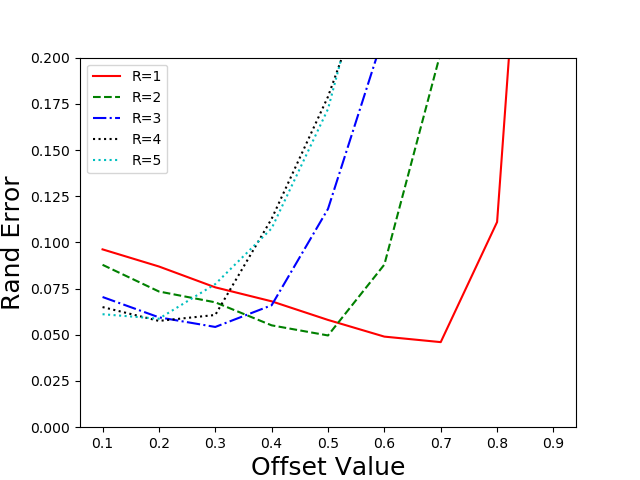
\includegraphics[height = 0.3\textheight]{offset_errors_verse_radius.png}
    \caption{Constrained correlation clustering result as a function of offset value with neighbors of different size. }
    \label{fig:offset_radius}
\end{figure}

\begin{figure}[h]
    \centering
    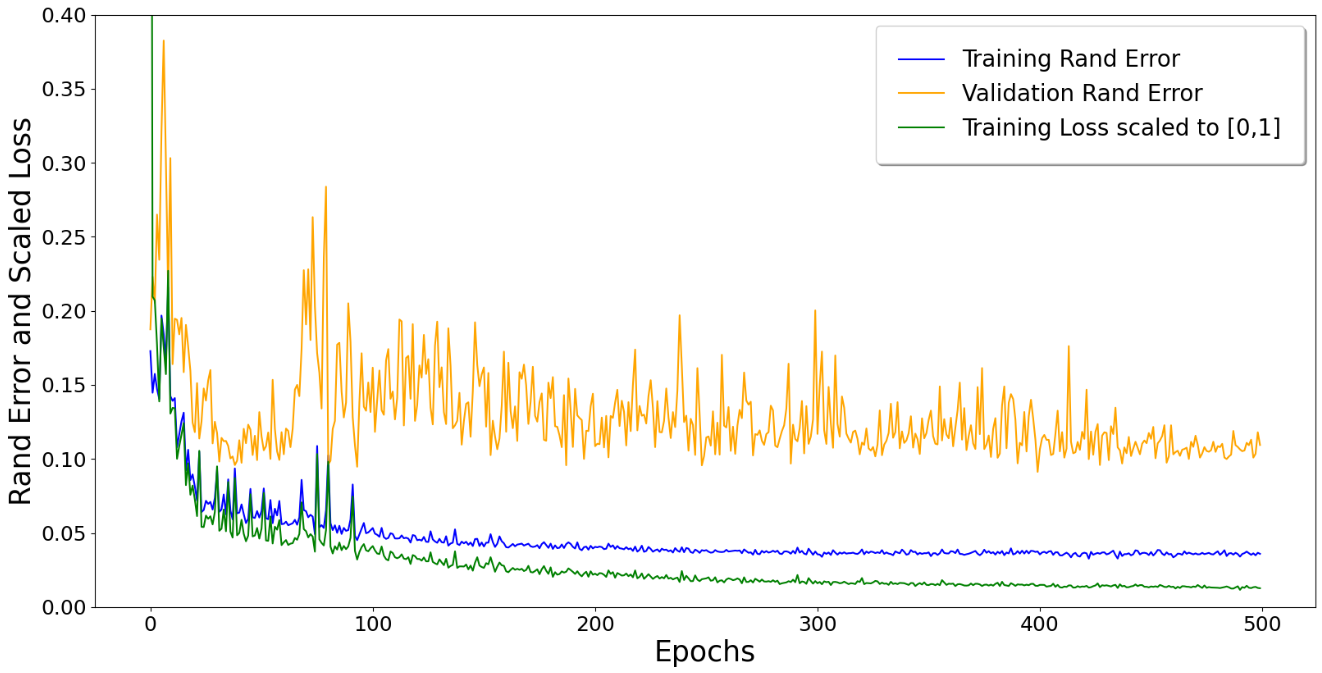
\includegraphics[height = 0.18\textheight]{run1crop.png}
    \caption{Run 1}
    \label{fig:run1}
\end{figure}



If we have time, we compare this to a waterfall hierarchy done with an MST.
\bibliographystyle{unsrt}  
\bibliography{references}  %%% Remove comment to use the external .bib file (using bibtex).
%%% and comment out the ``thebibliography'' section.


%%% Comment out this section when you \bibliography{references} is enabled.
\begin{biography}


Reid Porter is a research scientist at Los Alamos National Laboratory. His research interests include machine learning, signal processing, and computer architecture. Porter has a PhD in electrical engineering (199?) from the Queensland University of Technology, Australia.
%Beate Zimmer is an Associate Professor of Mathematics at Texas A\&M University--Corpus Christi and Guest Scientist at Los Alamos National Laboratory. She received her PhD in Mathematics from the University of Illinois - Urbana/Champaign in 1994.
%Quan Nguyen is currently pursuing a PhD in Computer Science at UT Arlington and earned an MS in Mathematics from Texas A\&M -Corpus Christi  in 2019.
%Venkatesh Jatla is pursuing PhD in Computer Engineering at the University of New Mexico. His Bachelors degree in Electrical and Computer Engineering was earned at Vellore Institute of Technology (2016).
\end{biography}


\end{document}


 
With respect to WS-CC hierarchies we make the following observations.
\begin{lemma} Any negative MST edge between two vertices that each border a positive MST edge is a watershed edge and gets cut.
\end{lemma}
\begin{proof}
If edge $A_{ij}<0$ and there are edges $e_{ki}, e_{jm}$ with $A_{ki}>0$ and , $A_{jm}>0$, then $A_{ij}^*>A_{ij}$ and the edge is not in a watershed basin.
\end{proof}

This means that a negative MST edge between two connected components would be  a watershed edge and be cut.

\begin{lemma} Any negative MST edge $e_{ij}$ that borders a positive MST edge $e_{ki}$  is a watershed basin edge if an only if all MST edges $e_{j,m}$ satisfy $A_{jm}<A_{ij}$.
\end{lemma}
\begin{proof}
In this case $ \max_{k\in N_i\setminus\{j\}}A_{ik}>A_{ij}$ and for a watershed basin edge we would need $A_{ij}>\min\left( \max_{k\in N_i\setminus\{j\}}A_{ik},\max_{k\in N_j\setminus\{i\}}A_{kj}\right)=\max_{k\in N_j\setminus\{i\}}A_{kj}$. If all MST edges on one side of edge $e_{ij}$ have lower affinities than $A_{ij}$ then the edge can not be a watershed edge.
\end{proof}

In the same scenario, if at least one  MST edge $e_{jm}$ satisfy $A_{jm}>A_{ij}$, then the edge is a watershed edge, as it is bordered by two MST edges with higher affinities.
